\chapter{Justificación}

	El agua es el recurso más valioso para los seres vivos de este planeta, por ello, el agotamiento y contaminación de este líquido es una amenaza para ecosistemas enteros y para las actividades humanas que dependen del agua. Dicho esto, se puede afirmar que la escasez de agua afecta todos los pilares de la sustentabilidad y esta carestía es cada vez más visible.
	
	A pesar de que en noviembre del 2002 el \acrfull{pidesc} otorgó en los artículos XI y XII a todos los seres humanos el derecho a contar con agua suficiente, a precio asequible, físicamente accesible, segura y de calidad aceptable para usos personales y domésticos \cite{fondo_para_la_comunicacion_y_la_educacion_ambiental_derecho_nodate}, la situación global no refleja el cumplimiento de ese derecho. El \acrfull{pnud} señala que la escasez de agua afecta a más del \qty{40}{\percent} de la población mundial \cite{pnud_objetivo_nodate} y se estima que esta cifra aumente drásticamente si no se emprenden las acciones necesarias para contrarrestar los factores que agravan el problema tales como el cambio climático, la contaminación de cuerpos acuosos y el crecimiento poblacional por mencionar algunos. La falta de agua arrastra consigo problemas sociales y de salud, entre los que se pueden mencionar:
		
	\begin{itemize}[columns=2]
		\item \textbf{Enfermedades:} Desde la falta de saneamiento hasta la ingesta de agua contaminada, la escasez de agua provoca el aumento de enfermedades entre las que se pueden incluir la diarrea, el cólera y la poliomielitis, sin mencionar la muerte por deshidratación.
		\item \textbf{Hambre:} La ganadería, agricultura y otras industrias son afectadas al no contar con agua, lo que puede llevar a la escasez de alimentos.
		\item \textbf{Desaparición de flora y fauna:} La falta de este recurso natural conlleva a la muerte y a veces extinción de los animales y plantas que dependían de un cuerpo de agua agotado.
		\item \textbf{Conflictos sociales:} Numerosos conflictos alrededor del mundo surgen por la falta de recursos y esto supone el desplazamiento forzado de las personas o incluso conflictos bélicos.
	\end{itemize}
	
	En mayo del 2021 la \acrfull{nasa} reportó que México afrontaba una sequía generalizada en aproximadamente \qty{85}{\percent} del territorio nacional, se reportó que cerca de 60 presas grandes se hallaban por debajo del \qty{25}{\percent} de su capacidad y como se muestra en la~\cref{fig:indice-estres-evaporativo} la sequía se concentró en el norte y centro del país. Pocos meses después, México ocupaba el puesto 24 de 164 en mayor estrés hídrico según una lista elaborada por el \acrshort{wri} \cite{efe_empeora_2021}, y de acuerdo al mismo organismo, para 2040 se situaría en la categoría de \textit{high-stress} \cite{maddocks_ranking_2015}, es decir, la segunda peor categoría.

	\begin{figure}[H]
		\centering
		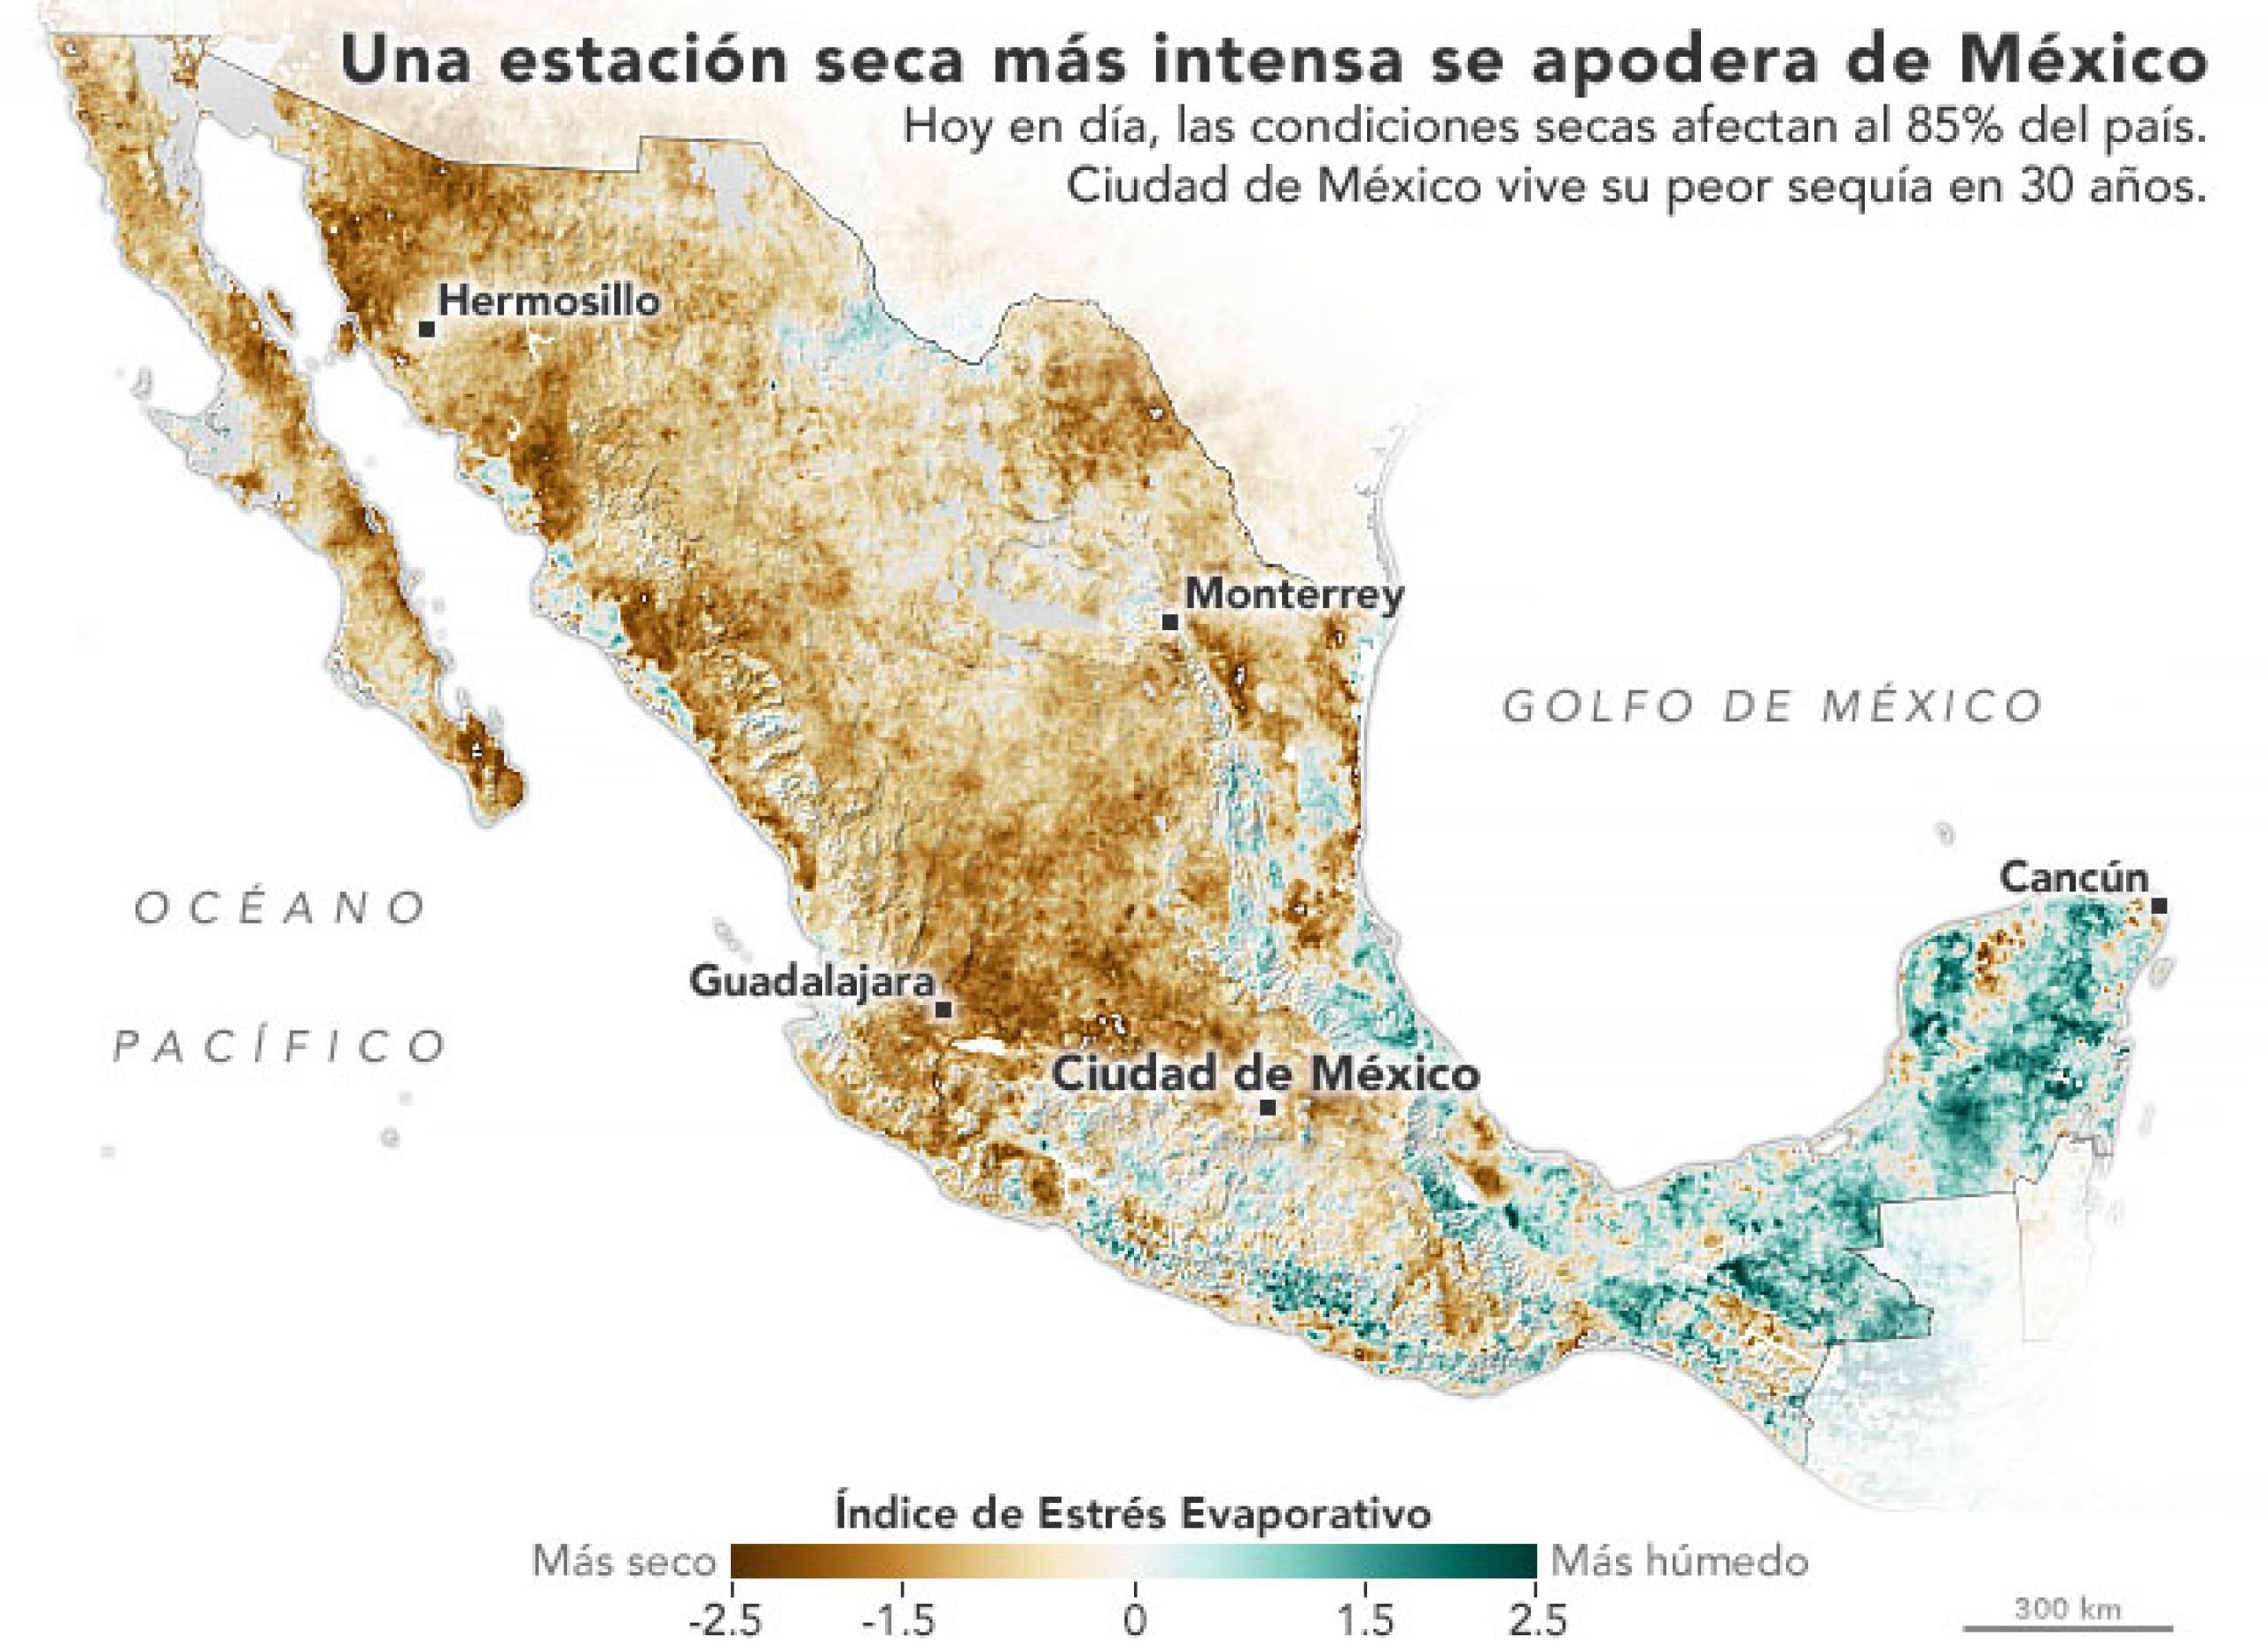
\includegraphics[width=\linewidth,height=70mm, keepaspectratio]{Justificación/indice-estres-evaporativo.jpg}
		\caption{Índice de estrés evaporativo}
		\floatfoot{Mapa obtenido de \cite{nasa_estacion_seca_mexico_2021}}
		\label{fig:indice-estres-evaporativo}
	\end{figure}
	
	México no es el único país que enfrenta esta crisis hídrica, de hecho, desde hace varios años, países han implementado políticas para el control y suministro seguro de agua, donde se halló en varias ocasiones una respuesta en la desalinización de agua; aquí es donde la destilación solar se abre camino como un sector de investigación para el suministro seguro, limpio y sustentable de agua.
	
	Varios estudios se han realizado para aumentar la productividad de la destilación solar. Se vislumbra entonces como un sector de investigación con grandes áreas de oportunidad para ser implementada a gran escala, pero para ello, el análisis de los procesos energéticos involucrados durante su operación resulta indispensable ya que uno de los problemas para implementar esta tecnología es el costo por cada litro producido y el reducir las pérdidas puede definir la viabilidad económica del proyecto.
	
%	La ciudad de Neon \cite{terra_mater_how_2021} representa un proyecto urbano que basa su suministro de agua en la \gls{desalinizacion} por medio de una torre esférica central de energía, 